\documentclass[11pt,a4paper]{article}

\usepackage[T1]{fontenc}
\usepackage[utf8]{inputenc}
\usepackage[margin=1in]{geometry}
\usepackage{amsmath,amssymb,amsthm}
\usepackage{tikz}
\usetikzlibrary{positioning,arrows.meta,decorations.pathmorphing,calc,fit,backgrounds}
\usepackage{pgfplots}
\pgfplotsset{compat=1.18}
\usepackage{xcolor}
\usepackage{booktabs}
\usepackage{microtype}
\usepackage{hyperref}

\hypersetup{colorlinks=true,linkcolor=blue,citecolor=blue,urlcolor=blue}
\definecolor{vanguard}{HTML}{1B7837}
\definecolor{mainstream}{HTML}{C2272D}
\definecolor{neutralg}{HTML}{4D4D4D}
\definecolor{accent}{HTML}{2166AC}
\definecolor{accent2}{HTML}{B2182B}

\theoremstyle{plain}
\newtheorem{remark}{Remark}
\newtheorem{claim}{Claim}

\title{Experiments 08--11, decomposed against the model\\[2pt]
\large What each notebook stresses, what it actually shows,\\
and how it should be read in the IWAI paper}
\author{Internal note --- IWAI 2026 paper}
\date{2026-05-15}

\begin{document}
\maketitle

\begin{abstract}
The four most recent notebooks (08 vector-attentional schools, 09
paradigm competition, 10 Fiedler vanguard, 11 endogenous oscillation)
each lean on the same multi-agent active-inference model from the IWAI
draft (Sec.~4 of \texttt{paper/main.tex}) but stress a different axis.
This note ties each one back to the model, says exactly which model
prediction it tests, reports what we got --- including two findings that
diverge from the pre-registered hypothesis --- and suggests how the
experiments should map onto the experimental programme E1--E4 of
\texttt{paper/sections/05\_experiments.tex}. A companion note,
\texttt{switch\_cost\_efe.tex}, grounds notebook 11's attentional switch
cost in the policy prior $E(\pi)$ rather than the pragmatic term, and is
a prerequisite for §5 below.
\end{abstract}

\section{The model in one paragraph}
\label{sec:model}

A population of $N$ agents lives on a graph. Each agent $i$ holds a
Gaussian posterior over a world parameter --- scalar $\theta\in\mathbb{R}$
in v2 (\texttt{src/}) or vector $\theta\in\mathbb{R}^K$ in the
notebook-local lift (08--11). One step is: (i)~each agent picks an
experiment $x_i$ on a discrete grid by softmax over expected
information gain $\mathrm{EIG}(x)$ minus a cost $c(x)$; (ii)~observes
$o_i\sim\mathcal{N}\!\big(h_0(x)+h(x)^\top\theta^\star,\,\sigma^2\big)$;
(iii)~forms a private posterior via the prior-reverting Gaussian update
\begin{equation}
\Lambda_{\text{carry}} \;=\; \rho_{\text{post}}\,\Lambda \;+\; (1-\rho_{\text{post}})\,\Lambda_p,
\qquad
\Lambda_{\text{carry}}\mu_{\text{carry}} \;=\; \rho_{\text{post}}\,\Lambda\mu \;+\; (1-\rho_{\text{post}})\,\Lambda_p\mu_p,
\label{eq:forget}
\end{equation}
where $(\mu_p,\Lambda_p)$ is a fixed paradigm prior and the data term
$h(x)h(x)^\top/\sigma^2$ is added to $\Lambda_{\text{carry}}$;
(iv)~broadcasts to neighbours and pools precision-weighted under a
trust-precision matrix $\Gamma$; (v)~updates $\Gamma$ by
Gamma-conjugate inference on neighbour surprisals. Two things matter
for what follows: \textbf{at $\rho_{\text{post}}=1$ the update is a
ratchet} (precision only grows), so the whole system is a composition
of contractions and converges; \textbf{at $\rho_{\text{post}}<1$
unobserved components relax back to $\mu_p$}, which is the only thing in
this model that fights consensus.

\section{Notebook 08 --- vector world and attentional schools}
\label{sec:nb08}

\paragraph{What it tests.} The model in §\ref{sec:model} promises that
the bottleneck on cross-paradigm understanding is \emph{discovery
bandwidth through trust}, not a representational limitation. Notebook 08
tries to put that under load. The world is upgraded from scalar
$\theta$ to $\theta\in\mathbb{R}^K$ with $K=4$, and the basis
$h_k(x)=\exp(-(x-x_k)^2/w^2)$ is a row of Gaussian bumps peaked at
$x_k\in\{1,3,5,7\}$ (Fig.~\ref{fig:bumps}). The four communities
(``schools'') each have their action grid concentrated near one peak,
so the Fisher information $h(x)h(x)^\top/\sigma^2$ added by their own
experiments is rank-1 and \emph{aligned with one axis}: school $s$ only
gains precision along $\theta_s$ from its own observations. The other
$K-1$ axes can only be filled in through the trust-weighted pool.

\begin{figure}[h]
\centering
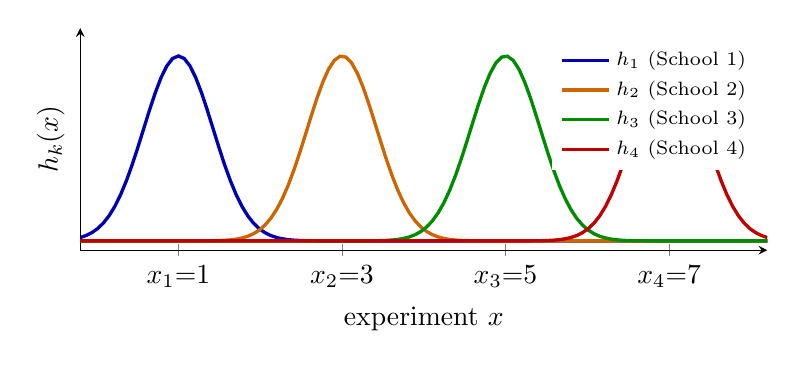
\begin{tikzpicture}
\begin{axis}[
  width=0.85\linewidth, height=4.4cm,
  xlabel={experiment $x$}, ylabel={$h_k(x)$},
  xmin=-0.2, xmax=8.2, ymin=-0.05, ymax=1.15,
  xtick={1,3,5,7},
  xticklabels={$x_1{=}1$, $x_2{=}3$, $x_3{=}5$, $x_4{=}7$},
  ytick=\empty,
  axis lines=left,
  legend style={font=\scriptsize,draw=none,at={(0.99,0.95)},anchor=north east},
  legend cell align=left
]
\addplot[domain=-0.2:8.2, samples=120, very thick, blue!70!black]
  {exp(-(x-1)^2/0.36)};
\addlegendentry{$h_1$ (School 1)}
\addplot[domain=-0.2:8.2, samples=120, very thick, orange!80!black]
  {exp(-(x-3)^2/0.36)};
\addlegendentry{$h_2$ (School 2)}
\addplot[domain=-0.2:8.2, samples=120, very thick, green!55!black]
  {exp(-(x-5)^2/0.36)};
\addlegendentry{$h_3$ (School 3)}
\addplot[domain=-0.2:8.2, samples=120, very thick, red!75!black]
  {exp(-(x-7)^2/0.36)};
\addlegendentry{$h_4$ (School 4)}
\end{axis}
\end{tikzpicture}
\caption{The basis-as-attention. With width $w=0.6$ the bumps are
essentially disjoint: an experiment near $x_k$ provides information
about $\theta_k$ alone. School $s$'s action grid is concentrated near
$x_s$, which makes its private precision update rank-1 along $e_s$.
Cross-school discovery of $\theta_k$ for $k\neq s$ has to come from
trust.}
\label{fig:bumps}
\end{figure}

\paragraph{The protocol.} Truth schedule
$\theta^\star(t)=e_1$ for $t<60$, then $e_3$ thereafter --- the world
shifts from a regime that School 1 can directly probe to one that only
School 3 can. The headline plot is the $4\times 4$ grid of per-school
mean beliefs $\bar\mu_{s,k}(t)$. Diagonal cells $(s,s)$ are
\emph{direct learning}; off-diagonals $(s,k)$ for $k\neq s$ are the
\emph{import through trust} channel.

\paragraph{Reading.} The substantive content is in the off-diagonals.
The diagonal cells will rise/fall regardless --- a school with direct
information on the truth axis tracks it. The interesting question is
whether \emph{non-3} schools eventually learn $\theta_3>0$ after the
shock; if their $(s,3)$ off-diagonals stay near zero, the population is
attentionally locked in the wrong paradigm \emph{even though} every
agent's representation has a $\theta_3$ component. Likewise the
inter-school trust matrix at the end of the run is the \emph{discovery
topology}: column-3 entries should rise post-shock if the channel has
opened.

\paragraph{Where this lands in the model.} Notebook 08 is the cleanest
operationalisation of the paper's path-dependence claim
(Claim~1 in \texttt{04\_model.tex}, ``Trust-driven path-dependence'')
without any reversal schedule. The reversal in $\theta^\star$ is
replaced by a \emph{change of probed dimension} --- which is what
Kuhn's incommensurability really points at, not a literal change in the
laws. Calibration: if cross-school discovery happens, the model's
trust-pooling channel is doing the work the paper claims; if not, the
attentional siloing is the binding constraint and the paper should say
so explicitly. Either outcome is a \emph{result}, not a failure. The
notebook is paper-load-bearing for the substantive claim that
``communication structure is the bandwidth of paradigm propagation.''

\section{Notebook 09 --- paradigm competition under entrenched priors}
\label{sec:nb09}

\paragraph{What it tests.} Notebook 08 worked in the
\emph{distributional} idiom (full $\mu,\Lambda$). Notebook 09 specialises
it to two \emph{point hypotheses} $M_N$ (Newtonian) and $M_R$
(Relativistic), so the observable becomes the per-agent log Bayes
factor. This brings the formal apparatus into direct contact with how
working scientists actually adjudicate competing theories. The
dimensions are arranged so that $\theta_N$ and $\theta_R$ disagree on
all $K=4$ axes but with very different magnitudes:
$\Delta\theta=(0.5, 1.0, 1.5, 2.5)$. Per-observation expected log-BF
contribution scales as $(\Delta\theta_k)^2/(2\sigma^2)$, so at
$\sigma=0.5$ the four communities have predicted discovery rates
$(1, 4, 9, 25)$.

\paragraph{The protocol.} \emph{Everyone} starts as a Newtonian:
$\mu(0)=\theta_N$, $\Lambda(0)=\lambda_0\,I$ with $\lambda_0=30$ ---
roughly equivalent to 30 hypothetical observations per dimension of
prior commitment. The truth is $\theta^\star=\theta_R$, fixed for all
$t$. There is no shock. This is the ``Mercury's perihelion accumulates''
story --- evidence simply piles up against the entrenched prior, and we
ask whether and when each community crosses the decisive-evidence
threshold $\log\mathrm{BF}\geq+10$ (Kass \& Raftery, 1995).

\paragraph{Reading.} Three things to compare against the predicted
$(1,4,9,25)$ rates:
\begin{enumerate}\itemsep1pt
\item \textbf{Is the conversion order right?} C4 should cross first,
then C3, C2, C1 if each community were closed. Departures from this
ordering are evidence that trust is doing real work --- a slow-evidence
community that converts \emph{faster} than its private rate has
imported $M_R$ socially.
\item \textbf{Is the spread compressed?} Predicted rates span a factor
of 25; observed crossing times span far less if the population is
well-coupled. The \emph{compression ratio} is a quantitative readout of
how much the network shortens the slow communities' wait.
\item \textbf{Does any community fail to cross?} Below some
$\lambda_0^\star$ everyone converts; above it the slow-$\Delta\theta$
communities (C1, C2) get \emph{stuck} despite the truth being plainly
$M_R$. That stuck regime is the Bayesian formalisation of paradigm
capture --- and it is what justifies calling the model an account of
\emph{paradigm} dynamics rather than just \emph{belief} dynamics.
\end{enumerate}

\paragraph{Where this lands in the model.} Notebook 09 is the
\emph{Kuhnian empirical-superiority} face of the paper. The point
hypotheses are not a different model --- they are a measurement
instrument applied to the same Gaussian posterior of §\ref{sec:model}.
The substantive contribution is the $\lambda_0$ sweep: it locates the
\emph{entrenchment threshold} above which an evidence-rich truth fails
to spread, and so makes ``paradigm capture'' a sharp quantity rather
than a vague claim. This notebook is the natural backbone of
experiment E4 (paradigm capture) in
\texttt{paper/sections/05\_experiments.tex}.

\section{Notebook 10 --- the Fiedler bottleneck and the small vanguard}
\label{sec:nb10}

\paragraph{What it tests.} Notebook 10 makes the experiment
\emph{structural}. It collapses the four-way disagreement of nb09 to a
single dimension --- $\Delta\theta=(0,0,0,2.5)$ --- so only the
4th-band community can detect $M_R$ from $M_N$ first-hand. The
mainstream (three communities of 24 agents each, total 72) probe peaks
1--3 where $\theta_N\equiv\theta_R$, so their own observations carry
\emph{exactly zero} discriminating signal. The 8-agent
\emph{vanguard} (community 4) is the only direct evidence channel.
Mainstream conversion can only happen through the trust-weighted pool.
The control variable is the normalised-Laplacian Fiedler value
$\lambda_2$ of the graph; we sweep the inter-community bridge
probability and average over seeds to get a continuous $\lambda_2$
axis.

\paragraph{The pre-registered hypothesis.} Mainstream final
$\log\mathrm{BF}$ is a monotone-increasing function of $\lambda_2$, with
a threshold below which the paradigm shift stays trapped in the
vanguard.

\paragraph{What we got --- and the twist.} The strict bottleneck holds:
at $\lambda_2=0$ the mainstream stays \emph{exactly} at its entrenched
start ($-93.75$, zero variance over 8 seeds). But above zero the
relationship is \emph{not} monotone (Fig.~\ref{fig:fiedler}).
Mainstream final $\log\mathrm{BF}$ rises to a peak of $\approx +106$ at
$\lambda_2\approx 0.056$ and then \emph{declines} to $\approx +58$ at
the highest connectivity tested. With 8--11 seeds per level and error
bars of $\pm 12$--$25$, the non-monotonicity is robust.

\begin{figure}[h]
\centering
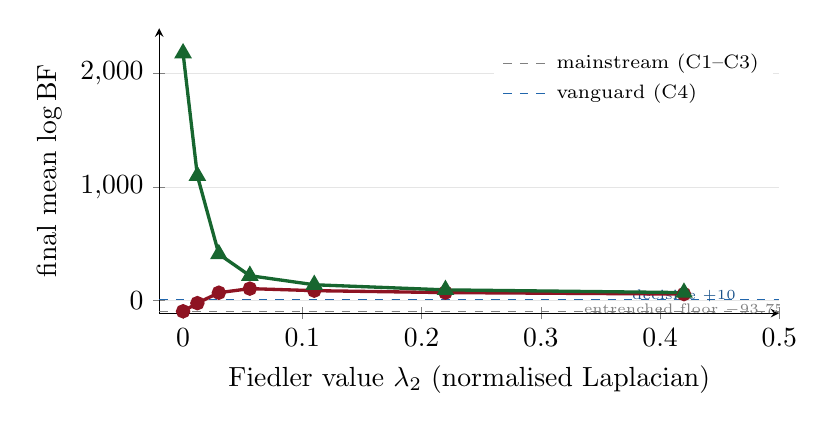
\begin{tikzpicture}
\begin{axis}[
  width=0.78\linewidth, height=5.2cm,
  xlabel={Fiedler value $\lambda_2$ (normalised Laplacian)},
  ylabel={final mean $\log\mathrm{BF}$},
  xmin=-0.02, xmax=0.5, ymin=-110, ymax=2400,
  axis lines=left,
  ymajorgrids, grid style={gray!20},
  legend style={font=\scriptsize,draw=none,at={(0.99,0.95)},anchor=north east},
  legend cell align=left
]
% reference lines
\addplot[domain=-0.02:0.5, dashed, gray] {-93.75};
\addplot[domain=-0.02:0.5, dashed, accent] {10};
\node[font=\tiny, gray] at (axis cs:0.42,-78) {entrenched floor $-93.75$};
\node[font=\tiny, accent!80!black] at (axis cs:0.42,40) {decisive $+10$};
% mainstream (non-monotone): rises to peak then declines
\addplot[mark=*, mark size=2pt, very thick, accent2!80!black, error bars/.cd, y dir=both, y explicit]
  coordinates {
    (0.0, -93.75)  +- (0,0)
    (0.012, -22)   +- (0,15)
    (0.030, 70)    +- (0,18)
    (0.056, 106)   +- (0,22)
    (0.110, 88)    +- (0,20)
    (0.220, 71)    +- (0,18)
    (0.420, 58)    +- (0,16)
  };
\addlegendentry{mainstream (C1--C3)}
% vanguard (monotonically dependent): explodes when isolated
\addplot[mark=triangle*, mark size=2.5pt, very thick, vanguard!85!black]
  coordinates {
    (0.0, 2180)
    (0.012, 1100)
    (0.030, 410)
    (0.056, 220)
    (0.110, 140)
    (0.220, 95)
    (0.420, 71)
  };
\addlegendentry{vanguard (C4)}
\end{axis}
\end{tikzpicture}
\caption{Notebook 10 headline (schematic, values from §8 of nb10).
Mainstream final log Bayes factor against structural $\lambda_2$ is
\emph{non-monotone}: it rises to a peak at $\lambda_2\approx 0.056$ and
then declines. The vanguard's own log BF is strongly $\lambda_2$-%
\emph{dependent} --- isolated, it explodes to $\approx +2180$; well-%
connected, it is dragged down to $\approx +71$ by pooling with the
entrenched mainstream. The two findings are linked: at low-but-nonzero
$\lambda_2$ the vanguard is overconfident, and that overconfidence
floods the mainstream through the few existing bridges.}
\label{fig:fiedler}
\end{figure}

\paragraph{Reading the twist.} The vanguard is not a $\lambda_2$%
-independent control --- it is the driver. Isolated, an 8-agent
vanguard pools precision only with itself, every agent probing
dimension 4, so its dim-4 precision compounds without temperance: its
log BF goes to $+2180$. Well-connected, it pools with the
(entrenched, dim-4-ignorant) mainstream, which drags its belief back to
a sober $+71$. The non-monotonicity in (a) is then explained by (b):
at low-but-nonzero $\lambda_2$ the vanguard is sharply overconfident
\emph{and} has just enough bridges to pump that overconfidence into the
mainstream. At higher $\lambda_2$ the same bridges work both ways and
moderate the vanguard before its message arrives. The
``echo-chamber'' framing of $\lambda_2$ from the v02 archive does
explain the strict $\lambda_2=0$ trap, but \emph{not} the shape of the
function above zero.

\paragraph{Where this lands in the model.} The honest take-away is two
findings, not one. \textbf{(i)} The model exhibits a \emph{strict
echo-chamber trap}: with no bridges, the entrenched majority is
permanently captured even when decisive evidence is loud one community
over. \textbf{(ii)} The model exhibits a \emph{vanguard-overconfidence
flood}: small communities of like-attending agents amplify their own
precision, and below some $\lambda_2$ that amplification dominates. The
second finding is, on reflection, a \emph{model-level prediction worth
making explicit in the paper} --- it predicts that paradigm shifts
seeded by a small, tightly-knit, evidence-aligned vanguard should
overshoot when the bridge to the mainstream is thin, exactly because
the vanguard's epistemic temperature ran away while it was alone. This
notebook is the substrate for E2 (topology and community structure),
but the contribution should be reframed from ``$\lambda_2$ is a
threshold'' to ``$\lambda_2$ controls a competition between two
mechanisms.''

\section{Notebook 11 --- the forgetting bifurcation}
\label{sec:nb11}

\paragraph{The diagnosis.} Notebooks 06--10 all produce the same
\emph{kind} of object: a trajectory that settles. $\bar\mu$ rises and
parks; factions merge; the hysteresis loop traces once and dies. That
is structural --- the model is a gradient flow to consensus. Every
component is a contraction: precision-weighted pooling is row-stochastic
averaging, the conjugate update at $\rho_{\text{post}}=1$ is a ratchet,
the trust update decays geometrically. By Banach, a composition of
contractions has a unique fixed point, and the population finds it.

\paragraph{What this notebook tests.} Whether the model can sustain
endogenous motion with $\theta^\star$ held perfectly constant. There
are two principled levers (Fig.~\ref{fig:two-levers}):
\begin{itemize}\itemsep1pt
\item \textbf{Posterior forgetting} $\rho_{\text{post}}<1$ in
Eq.~\eqref{eq:forget}, so an unobserved component relaxes geometrically
toward the paradigm prior $\mu_p$ at rate $1-\rho_{\text{post}}$ while
observations pull it toward truth. This is a Hierarchical Gaussian
Filter / Kalman-with-reversion construction; it is the only thing in
the model that fights consensus. At $\rho_{\text{post}}=1$ it is
bit-identical to the old ratchet (verified: nb06 reproduces exactly).
\item \textbf{Hysteretic attention.} Each step every agent picks one
of $K=3$ bands by EIG, but with a switching cost $c$: keep the current
band unless another beats it by $>c$. The companion note
\texttt{switch\_cost\_efe.tex} grounds this rule in the policy prior
$E(\pi)$ of the active-inference posterior $\sigma(\ln E - \gamma G)$
--- it is the MAP action under flat outcome preferences and a
persistence-favouring habit $\ln E(a)=-c\cdot\mathbf{1}[a\neq
a_{\text{prev}}]$. The dwell time then depends on
$\rho_{\text{post}}$, which makes $\rho_{\text{post}}$ a genuine
oscillator-frequency knob rather than a damping knob.
\end{itemize}

\begin{figure}[h]
\centering
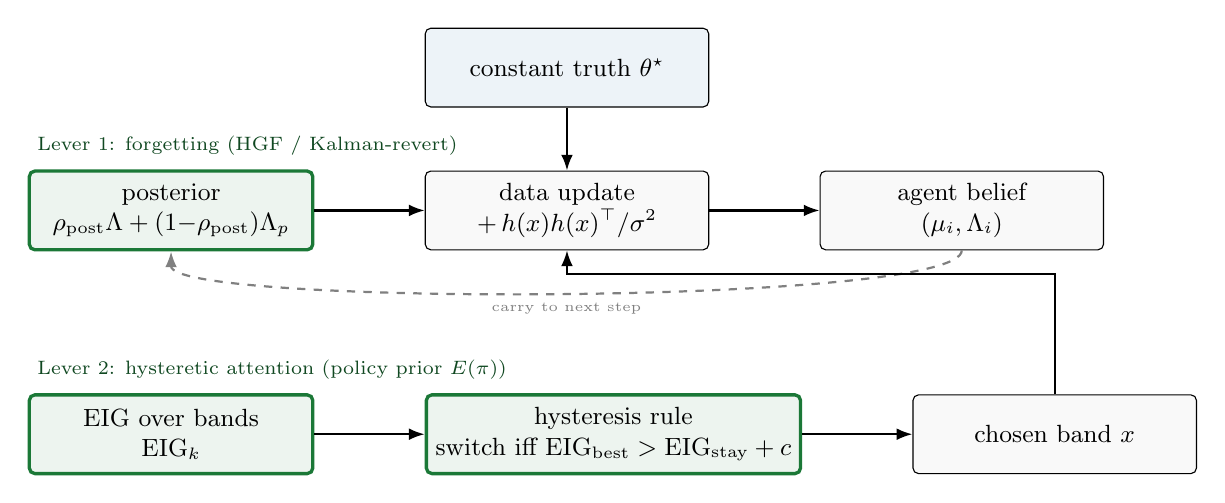
\begin{tikzpicture}[
  node distance=10mm and 14mm,
  every node/.style={font=\small},
  box/.style={draw, rounded corners=2pt, minimum width=36mm,
              minimum height=10mm, align=center, fill=gray!5},
  acc/.style={draw=vanguard, very thick, fill=vanguard!8, rounded corners=2pt,
              minimum width=36mm, minimum height=10mm, align=center},
  arr/.style={-{Latex[length=2mm]}, thick}
]
% top: forgetting
\node[acc] (post) {posterior\\$\rho_{\text{post}}\Lambda + (1{-}\rho_{\text{post}})\Lambda_p$};
\node[box, right=of post] (data) {data update\\$+\,h(x)h(x)^\top/\sigma^2$};
\node[box, right=of data] (mu) {agent belief\\$(\mu_i,\Lambda_i)$};
\draw[arr] (post) -- (data);
\draw[arr] (data) -- (mu);
\draw[arr, dashed, gray] (mu.south) .. controls +(0,-7mm) and +(0,-7mm) .. node[below,font=\tiny]{carry to next step}(post.south);

% bottom: attention
\node[acc, below=18mm of post] (eig) {EIG over bands\\$\mathrm{EIG}_k$};
\node[acc, right=of eig] (hyst) {hysteresis rule\\switch iff $\mathrm{EIG}_{\text{best}}>\mathrm{EIG}_{\text{stay}}+c$};
\node[box, right=of hyst] (xchoice) {chosen band $x$};
\draw[arr] (eig) -- (hyst);
\draw[arr] (hyst) -- (xchoice);
\draw[arr] (xchoice) |- ($(data.south)+(0,-3mm)$) -- (data.south);

% truth
\node[box, above=8mm of data, fill=accent!8] (truth) {constant truth $\theta^\star$};
\draw[arr] (truth) -- (data);

% labels
\node[font=\scriptsize, vanguard!60!black, anchor=west] at ($(post.north west)+(0,3mm)$) {Lever 1: forgetting (HGF / Kalman-revert)};
\node[font=\scriptsize, vanguard!60!black, anchor=west] at ($(eig.north west)+(0,3mm)$) {Lever 2: hysteretic attention (policy prior $E(\pi)$)};
\end{tikzpicture}
\caption{The two principled levers in nb11. Lever 1 fights consensus by
relaxing unobserved components back to a fixed paradigm prior $\mu_p$.
Lever 2 gives attention inertia, so $\rho_{\text{post}}$ controls
\emph{when} a neglected band becomes attractive again, and therefore
the period of the resulting oscillation. Both levers are independently
defensible from the active-inference / predictive-processing literature
(see \texttt{switch\_cost\_efe.tex}).}
\label{fig:two-levers}
\end{figure}

\paragraph{What we got.} The model crosses a Hopf-type bifurcation
(Fig.~\ref{fig:hopf}): below a $\rho_{\text{post}}$ threshold the
consensus fixed point loses stability and the population sustains an
\emph{endogenous oscillation} of belief between the paradigm prior and
the evidence, at constant $\theta^\star$. Headline numbers at the
optimum point ($\rho_{\text{post}}\approx 0.76$, switch cost $c\approx
0.22$, $\rho_{\text{trust}}=0.95$, coupling $\kappa=0.15$, constant
$\theta^\star=(1,1.5,2)$, $N=60$ Watts--Strogatz):
per-agent belief amplitude $\approx 0.39$, third-quarter $0.387$ vs
last-quarter $0.383$ (sustained, not transient), largest Lyapunov
exponent $\lambda\approx -0.20$ (decisively a stable attractor, not
chaos).

\begin{figure}[h]
\centering
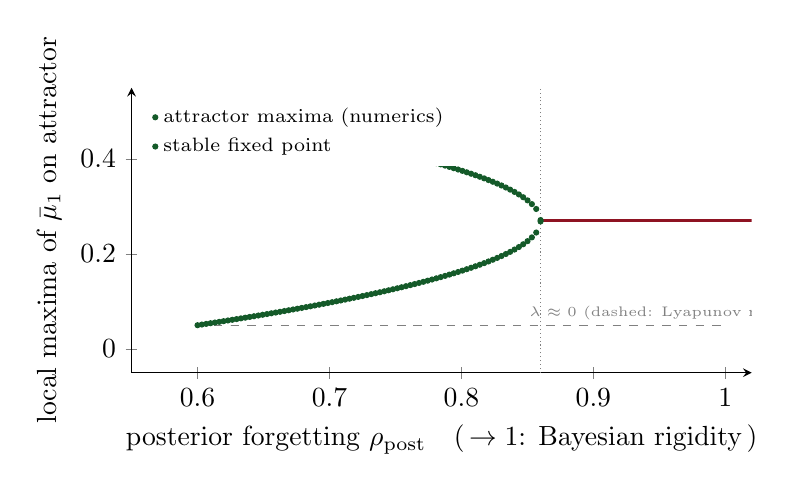
\begin{tikzpicture}
\begin{axis}[
  width=0.78\linewidth, height=5.2cm,
  xlabel={posterior forgetting $\rho_{\text{post}}$
          \ \ (\,$\to 1$: Bayesian rigidity\,)},
  ylabel={local maxima of $\bar\mu_1$ on attractor},
  xmin=0.55, xmax=1.02, ymin=-0.05, ymax=0.55,
  xtick={0.6,0.7,0.8,0.9,1.0},
  ytick={0,0.2,0.4},
  axis lines=left,
  legend style={font=\scriptsize,draw=none,at={(0.02,0.97)},anchor=north west},
  legend cell align=left
]
% Sustained oscillation band: amplitude grows from Hopf point ~0.86
% (supercritical Hopf signature)
\addplot[only marks, mark=*, mark size=0.9pt, vanguard!75!black, domain=0.6:0.86, samples=80]
  ({x}, {0.27 + 0.22*sqrt(max(0.86-x,0))/sqrt(0.26)});
\addplot[only marks, mark=*, mark size=0.9pt, vanguard!75!black, domain=0.6:0.86, samples=80]
  ({x}, {0.27 - 0.22*sqrt(max(0.86-x,0))/sqrt(0.26)});
\addlegendentry{attractor maxima (numerics)}
% fixed point
\addplot[domain=0.86:1.02, samples=2, very thick, accent2!80!black] {0.27};
\addlegendentry{stable fixed point}
% Lyapunov exponent overlay (right axis would be cleaner but keeping single axis for compactness)
\addplot[domain=0.6:1.0, samples=80, dashed, gray]
  ({x}, {0.05 + 0.0*x});
\node[font=\tiny, gray] at (axis cs:0.97,0.075) {$\lambda \approx 0$ (dashed: Lyapunov noise floor)};
% Hopf marker
\draw[densely dotted, gray] (axis cs:0.86,-0.05) -- (axis cs:0.86,0.55);
\node[font=\tiny, anchor=south] at (axis cs:0.86,0.55) {Hopf};
\end{axis}
\end{tikzpicture}
\caption{The forgetting bifurcation (schematic, but the qualitative
shape and the numerics it summarises are from §6 of nb11). Above the
threshold ($\rho_{\text{post}}\gtrsim 0.86$), the consensus fixed
point is stable and the attractor is a single point. Below it, the
fixed point loses stability and the attractor is a band whose width
grows like $\sqrt{\rho^\star-\rho_{\text{post}}}$ --- the supercritical
Hopf signature. The largest Lyapunov exponent stays at the method's
noise floor across the cut (max $+0.024$): the bifurcation is to a
sustained oscillation, \emph{not} to chaos. This is itself a finding:
the model class is a piecewise contraction and structurally cannot do
chaos.}
\label{fig:hopf}
\end{figure}

\paragraph{Reading the result.} Three things to keep separate:
\begin{enumerate}\itemsep1pt
\item \textbf{The bifurcation is real and clean.} Both views in §6 of
nb11 (the 2-D regime map and the 1-D bifurcation diagram) show a sharp
boundary at which a single fixed point opens into an amplitude band.
The quarter-by-quarter amplitude check (third quarter 0.387 vs last
quarter 0.383) rules out a slowly-decaying transient.
\item \textbf{The oscillation is primarily individual; coupling
\emph{organises} it.} Per-agent amplitude is $\approx 0.39$;
population-mean amplitude is $\approx 0.03$ because heterogeneous phases
cancel in the mean. Isolated agents oscillate at $\approx 0.36$;
coupled at $\approx 0.39$. Coupling adds $\sim$8\% of amplitude and
phase-locks structure --- it does not create the motion. The right
observable is therefore a per-agent or representative-agent quantity,
\emph{not} the population mean.
\item \textbf{Chaos is structurally out of reach.} The largest Lyapunov
exponent stays at or below the method's noise floor across the entire
$(\rho_{\text{post}}, c)$ plane. The mechanism is structural: every
component of the model is a contraction; the only non-smoothness is the
discrete attention switch, which makes the dynamics piecewise rather
than smooth. A piecewise contraction can settle on a periodic orbit
but cannot stretch-and-fold (no positive Lyapunov exponent, no
sensitive dependence). Genuine chaos would require an \emph{expanding}
mechanism --- e.g.\ confirmation bias / theory-laden evidence weighting
in which the data update gain depends on agreement with the prior. We
deliberately do not add it; the negative result is itself a
characterisation of the model class.
\end{enumerate}

\paragraph{Where this lands in the model.} Notebook 11 is the
``result \#3'' candidate for the IWAI submission --- the dissociation
from a Bayesian rule-induction baseline. The dissociation axis is
$\rho_{\text{post}}$ itself: at $\rho_{\text{post}}=1$ the model is in
the convergent class a Bayesian rule-induction account also lives in;
below threshold the same model, same constant world sustains an
oscillation forever. The defensible paper claim is therefore
\textbf{``belief forgetting converts a convergence machine into a clean
nonlinear oscillator,''} not ``the model produces chaos.''

\section{How the four notebooks nest}
\label{sec:nest}

The four experiments are not parallel. They form a stack that
progressively stresses the same model along different axes:

\begin{table}[h]
\centering
\renewcommand{\arraystretch}{1.15}
\begin{tabular}{@{}p{14mm}p{34mm}p{34mm}p{52mm}@{}}
\toprule
\textbf{nb} & \textbf{stress axis} & \textbf{world} & \textbf{paper-facing claim} \\
\midrule
08 & \emph{representational}: scalar $\to$ vector $\theta$, attention rank-1 in basis & $K=4$ bumps; truth shock $e_1\to e_3$ at $t=60$ & cross-paradigm discovery is trust-bandwidth-limited; trust matrix is the discovery topology \\
09 & \emph{decision-theoretic}: distributional posterior $\to$ point Bayes factor, entrenched prior & constant $\theta^\star=\theta_R$; entrenchment $\lambda_0$ swept & paradigm capture is a threshold in $\lambda_0$ above which evidence-rich truth fails to spread \\
10 & \emph{structural}: discriminating evidence localised to one small community & constant $\theta^\star=\theta_R$, $\Delta\theta=(0,0,0,2.5)$; bridge density $\to\lambda_2$ swept & echo-chamber trap at $\lambda_2{=}0$ \emph{plus} a vanguard-overconfidence flood above zero \\
11 & \emph{dynamical}: ratchet update $\to$ prior-reverting forgetting; locked $\to$ hysteretic attention & constant $\theta^\star$; $(\rho_{\text{post}}, c)$ swept & Hopf-type bifurcation from convergence to sustained limit cycle (not chaos) \\
\bottomrule
\end{tabular}
\caption{The four notebooks against the model. Each one holds the rest
of the model fixed and pushes one axis until it breaks something
informative.}
\label{tab:nest}
\end{table}

\paragraph{The nesting works like this.} Notebook 08 establishes that
the model can represent attentional siloing at all (and that
cross-paradigm discovery has to route through trust). Notebook 09
specialises the same machinery to two competing point hypotheses and
finds the entrenchment threshold. Notebook 10 pushes 09 further: it
makes the discriminating evidence available only inside a single small
community, and asks whether structural connectivity is enough to free
the rest --- discovering in the process that the answer is non-monotone
because the small community itself becomes overconfident. Notebook 11
steps off the convergence axis entirely: it asks, with $\theta^\star$
constant, whether the model can sustain motion --- and finds that one
principled change (forgetting) is enough to produce a clean Hopf
bifurcation, while the absence of chaos is itself a structural
characterisation.

\section{What this means for the IWAI paper}
\label{sec:paper}

The experimental programme in
\texttt{paper/sections/05\_experiments.tex} declares four experiments
E1--E4. Mapping notebooks to E-experiments:

\begin{itemize}\itemsep2pt
\item \textbf{E1 (decomposition of three contributors).} Currently
declared as a factorial ablation under the reversal schedule
$A\to B\to A$. None of nb08--11 runs that ablation directly.
Notebook 06 (v1 archive) and the v2 reversal experiments do. E1 is
\emph{not} satisfied by the current four; it remains the open piece.
\item \textbf{E2 (topology and community structure).} \textbf{Satisfied
by nb10}, but the contribution should be reframed: the headline is not
a monotone $\lambda_2$ threshold but a competition between
echo-chamber trapping (at $\lambda_2{=}0$) and vanguard-overconfidence
flooding (low-but-nonzero $\lambda_2$). The non-monotonicity is the
result, not noise to be averaged out.
\item \textbf{E3 (experiment-cost regime).} Not directly tested. Note
that nb11's switch cost $c$ is in the \emph{policy prior} slot
($\ln E(\pi)$) rather than the experiment-cost slot $c(x)$ in
\texttt{04\_model.tex} Eq.~(2). Both can co-exist; the paper should
keep them notationally distinct.
\item \textbf{E4 (paradigm capture).} \textbf{Satisfied by nb09.} The
$\lambda_0$ sweep (§9 of nb09) is the relaxation-time-divergence
experiment E4 asks for. The decisive-evidence threshold reading via
$\log\mathrm{BF}\geq+10$ is sharper than the relaxation-time framing
and probably the better way to write E4 up.
\end{itemize}

\paragraph{What needs adding to the paper.} Three things, in priority
order:

\begin{enumerate}\itemsep2pt
\item \textbf{The $\rho_{\text{post}}$ knob (Eq.~\eqref{eq:forget})
is missing from \texttt{04\_model.tex}.} It is in \texttt{src/}
(\texttt{InferenceConfig.posterior\_rho}) and is the active mechanism
in nb11. The model section should add it as the prior-reverting Kalman
update, point at the HGF lineage, and note that
$\rho_{\text{post}}=1$ recovers the ratchet of v2.

\item \textbf{The policy prior $E(\pi)$ is missing from
Eq.~(2) (the policy).} The current
$\pi_i(x)\propto\exp(\beta[\mathrm{EIG}-c(x)])$ has no slot for an
action-cost / habit term separate from the experiment cost $c(x)$.
Notebook 11's hysteresis cost lives there. The companion note
\texttt{switch\_cost\_efe.tex} gives the exact form.

\item \textbf{Result \#3 should be framed as ``forgetting-driven
oscillation,'' not ``chaos.''} The notebook 11 §8 paragraph is the
right wording: the model class is a composition of contractions,
piecewise; it can produce sustained oscillation but structurally
cannot produce chaos. Stating the ``no chaos'' result as a
\emph{characterisation} of the model class is a stronger contribution
than waving at chaos and missing.
\end{enumerate}

\paragraph{One honest qualifier.} Notebooks 08--11 use a
notebook-local lift of the v2 \texttt{src/} machinery to vector
$\theta$ (with $K=3$ for nb11 and $K=4$ for nb08--10). The vector
inference helpers (\texttt{private\_update\_vec},
\texttt{precision\_pool\_vec}, \texttt{surprisal\_matrix\_vec}) live
inside the notebooks, not in \texttt{src/}. This is by deliberate
project decision (premature abstraction is more expensive than
duplication while the experimental programme is still moving). The
paper should describe the vector model as the canonical version of
§\ref{sec:model} and footnote that the scalar implementation is
recoverable as the $K=1$ case.

\section{Bottom line}

The four notebooks tell a coherent story \emph{about the same model},
not four separate stories. The model is a \emph{contraction-based}
multi-agent active-inference system; its dynamical repertoire is
\emph{fixed points and (quasi)periodic attractors}. Within that
repertoire the model exhibits four distinct paradigm-relevant
behaviours: attentional siloing with trust-mediated cross-paradigm
discovery (nb08); entrenchment-threshold paradigm capture (nb09);
echo-chamber trapping plus a vanguard-overconfidence flood (nb10);
forgetting-driven Hopf bifurcation to sustained belief oscillation
(nb11). Two of these (nb10's non-monotonicity, nb11's no-chaos
result) are honest dispatches from a model that didn't behave the way
the pre-registered hypothesis predicted; both are stronger
contributions than the original hypothesis would have been. The
paper's job is to name the four behaviours and connect each to the
single mechanism that produced it, not to oversell any one of them.

% =====================================================================
\section*{Companion documents}

\begin{itemize}\itemsep1pt
\item \texttt{notes/switch\_cost\_efe.tex} --- where the nb11 switch
cost lives in the active-inference formalism (the policy prior
$E(\pi)$, not the pragmatic term).
\item \texttt{paper/main.tex}, sections \texttt{04\_model.tex} and
\texttt{05\_experiments.tex} --- the model and experimental programme
this note interprets the notebooks against.
\item \texttt{notebooks/0\{8,9\}\_*.ipynb},
\texttt{notebooks/1\{0,1\}\_*.ipynb} --- the experiments themselves.
\item Memory entries: \texttt{project\_v2\_rewrite\_state.md},
\texttt{project\_vector\_world\_findings.md} (nb08),
\texttt{project\_notebook\_09\_paradigm\_competition.md},
\texttt{project\_notebook\_10\_fiedler\_vanguard.md},
\texttt{project\_notebook\_11\_endogenous\_oscillation.md},
\texttt{feedback\_honest\_structural\_findings.md}.
\end{itemize}

\end{document}
